\documentclass[letterpaper,10 pt,conference]{ieeeconf}  % Comment this line out if you need a4paper

%\documentclass[a4paper, 10pt, conference]{ieeeconf}      % Use this line for a4 paper

\IEEEoverridecommandlockouts                              % This command is only needed if 
                                                          % you want to use the \thanks command

\overrideIEEEmargins                                      % Needed to meet printer requirements.

%In case you encounter the following error:
%Error 1010 The PDF file may be corrupt (unable to open PDF file) OR
%Error 1000 An error occurred while parsing a contents stream. Unable to analyze the PDF file.
%This is a known problem with pdfLaTeX conversion filter. The file cannot be opened with acrobat reader
%Please use one of the alternatives below to circumvent this error by uncommenting one or the other
%\pdfobjcompresslevel=0
%\pdfminorversion=4

% See the \addtolength command later in the file to balance the column lengths\documentclass{article}
% on the last page of the document

% The following packages can be found on http:\\www.ctan.org
\usepackage{graphics} % for pdf, bitmapped graphics files
\usepackage{epsfig} % for postscript graphics files
\usepackage{mathptmx} % assumes new font selection scheme installed
\usepackage{mathrsfs}
\usepackage{times} % assumes new font selection scheme installed
\usepackage{amsmath} % assumes amsmath package installed
\usepackage{amssymb}  % assumes amsmath package installed
\usepackage{caption}
\usepackage{gensymb}
\usepackage{graphicx,subfigure}
\usepackage{float}

\usepackage{hyperref}
\usepackage{cite}
\hypersetup{hypertex=true, 
	colorlinks=true,
	linkcolor=red,
	anchorcolor=red,
	citecolor=red,
    }

\title{\LARGE \bf
DirectionNet: Road Main Direction Estimation for Autonomous Vehicles from LiDAR Point Clouds*
}


\author{Wancheng Shen$^{1}$, Meiping Shi$^1$ and Tao Wu$^{1, \dag}$% <-this % stops a space
\thanks{*This work was not supported by any organization}% <-this % stops a space
\thanks{$^{1}$Wancheng Shen, Meiping Shi and Tao Wu are with the college of Intelligence Science and Technology, National University of Defense Technology, Changsha, China
        {\tt\small 14752276852@163.com; mp-shi@nudt.edu.cn; wutao@nudt.edu.cn}}%
\thanks{$^\dag$Corresponding Author.}
}


\begin{document}
\captionsetup[figure]{labelformat={default},labelsep=period,name={Fig.},font={small}}


\maketitle
\thispagestyle{empty}
\pagestyle{empty}


%%%%%%%%%%%%%%%%%%%%%%%%%%%%%%%%%%%%%%%%%%%%%%%%%%%%%%%%%%%%%%%%%%%%%%%%%%%%%%%%
\begin{abstract}

In recent years, ``end-to-end" autonomous driving methods based on deep learning have received increasing attention. Most of these methods take raw sensor data as input and directly generate vehicle control commands. The autonomous driving system is so complex that overfitting is inevitable, which will seriously affect the robustness and safety of the entire system. Although deep learning has shown outstanding performance over traditional machine learning in many tasks including environment perception, using end-to-end technologies that lack explanatory in the autonomous driving system will reduce system's robustness and safety. Different from existing perception tasks, inspired by human's driving style, we extract the key points of global route planning's projection on roads, which is called the ``road main direction". This ``road main direction" is then used for the subsequent driving tasks, guiding the vehicle along the road. Instead of using image as input, which is very susceptible to weather and illumination, our model directly processes the LiDAR point clouds. The results show that our method can extract the main direction of the road in different scenarios to provide direction guidance for the unmanned vehicle without a prior high-definition map.

\end{abstract}


%%%%%%%%%%%%%%%%%%%%%%%%%%%%%%%%%%%%%%%%%%%%%%%%%%%%%%%%%%%%%%%%%%%%%%%%%%%%%%%%
\section{INTRODUCTION}

After decades of development, autonomous driving technology can be mainly divided into two categories, one is based on traditional methods and supplemented by deep learning, and the other is based on deep learning, which has received extensive attention from researchers in recent years. The second method, so called end-to-end method, predicting control commands directly from raw sensor data using neural networks\cite{1,2,3,4,5}.

Conventional pipeline of autonomous driving generally consists of modules such as mapping, localization, perception, route planning and motion planning. Each component of this pipeline is fully developed, and this pipeline is used by many self-driving companies, which has been proven to be stable and effective. However, this pipeline is highly dependent on precise localization information provided by high-definition (HD) maps, which are expensive to build and maintain. When the driving environment of the vehicle changes, but the prior HD map is not updated in time, the localization information will be deviated and affecting the subsequent driving tasks, even the safety of the entire system.

Different from traditional approaches, the end-to-end approach aims to avoid building the maps of the environment and the subsequent localization and planning, collapsing the problem with a single neural network\cite{4}. This makes the autonomous driving system simple and efficient. Just feeding one image captured by the camera, the neural network will output the optimizing control commands, then the unmanned vehicle will move to the goal points without the map.

However, for the autonomous driving system, which is full of complexity and uncertainty, it is very difficult to use a single neural network to implement all these tasks perfectly. The mapping function that the neural network needs to learn will be very complex and requires huge training data to cover driving variations. The training process of the model will also become extremely difficult, and it will take a long time for the loss to converge. Inevitably, the model will overfit to a certain extent, which leads to low generalization, and the performance of the model will greately degrade if the vehicle enters a completely alien environment.

More importantly, using a single neural network to replace all the modules in the traditional pipeline will greatly reduce the security redundancy of the driving system, which is the critical factor in the automatic driving. In the traditional way, if the pre-order module, such as localization or perception deviates, the subsequent planning and control modules will try to make up for it to increase the security of the system. But in the end-to-end way, a small error can induce severe consequence. For example, when we reproduced the work called BADGR\cite{6}, we found that the model would erroneously consider shadows under tree canopies as impassable areas to avoid and drive off the normal road to rush towards the lawn, which would be dangerous if there were people on the lawn.

In summary, we believe that the role of deep learning is too small in traditional autonomous driving methods, but greatly exaggerated in the ``end-to-end" methods. In this paper we try to find an intermediate way to transition from traditional methods to end-to-end methods to fully exploit the strengths of deep learning. For the tasks of obstacle avoidance, local planning and vehicle control, there are already well-established solutions based on traditional methods, deep learning should be used for problems that are difficult to model with traditional methods, such as perception tasks. Different from existing perception tasks, inspired by human's driving style, we extract the "main direction" of the road from sensor data. An overview of the proposed approach is shown in Fig. \ref{overview}.

\begin{figure*}
	\centering
	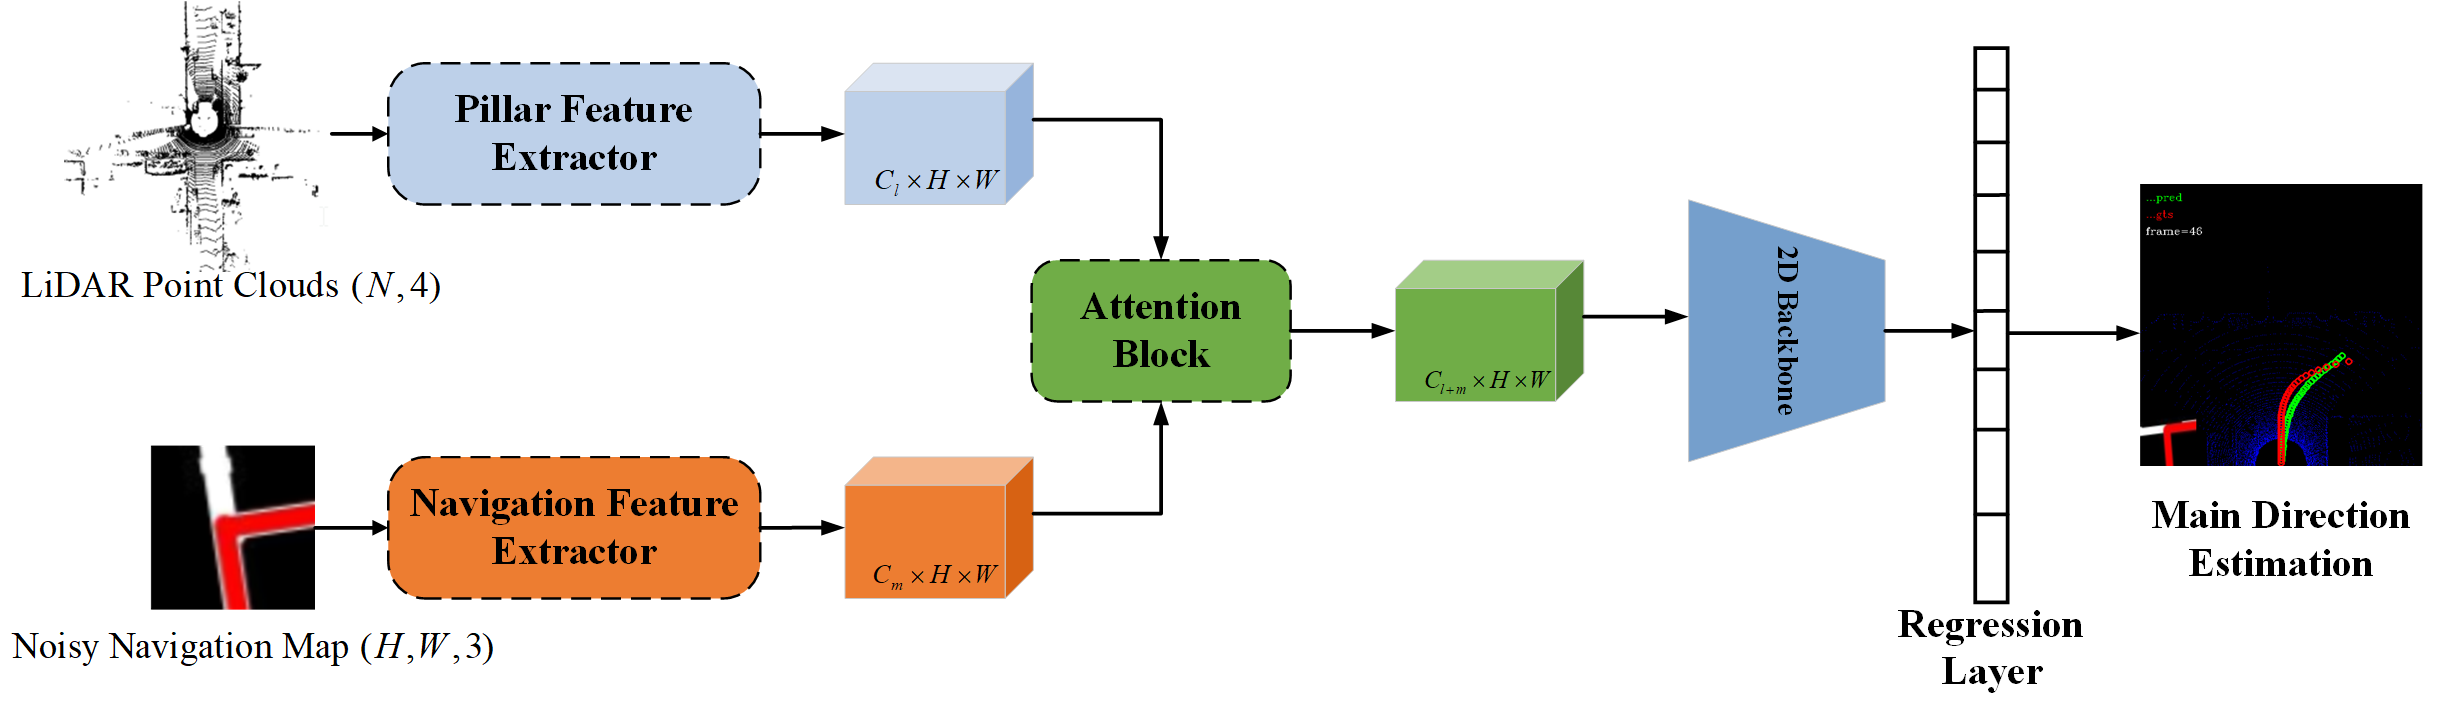
\includegraphics[width=0.7\linewidth]{../imgs/overview.png}
	\caption{\textbf{System overview:} DirectionNet takes LiDAR point clouds and local navigation map as input to estimate the main direction of the road. Using a Pillar Feature Extractor to extract the feature of the point clouds and then fused with the navigation map feature through the Attention Block. Finally a 2D backbone extracting high-level feature map followed by a full-connected layer to regress the length and y-coordinates representing the road main direction}
    \label{overview}
\end{figure*}

We analyze in-depth the process of human drivers driving to the destination under the guidance of a simple navigation map: driving along the road, avoiding obstacles, overtaking or other driving actions, and then continue to drive along the road, so, the main direction of the road is a very important information for the driver. Instead of using image as input, which is very susceptible to weather and illumination, our model directly processes the LiDAR point clouds. The "road main direction" is then used for the subsequent driving tasks, guiding the vehicle along the road. 

The rest of this paper is organized as follows. In Section \ref{related}, we introduce some related works. Section \ref{methods} provides an overview of the proposed approach. In Section \ref{experiments}, experimental results are presented. Finally, the conclusions are summarized in Section \ref{conclusions}.

\section{RELETED WORK}\label{related}

The conventional pipeline of autonomous driving typically consists of modules such as mapping and localization\cite{7,8,9}, perception\cite{10,11,12,13,14}, route planning and motion planning\cite{15,16,17}, control\cite{18,19}. This map-based method of autonomous driving relies heavily on offline-created HD maps using either LiDAR and/or vision. But it is expensive to build and maintain these HD maps. In order to reduce the operating cost of the system and improve the efficiency, there have been many learning-based methods to address these limitations by learning from data. In this section, we give a brief review of several popular learning-based systems, each with a different system design.

\subsection{Reinforcement Learning}

Reinforcement learning is a kind of experiential learning, it allows the agent to continuously explore and develop the environment based the reward. Reinforcement learning is often used in visual navigation tasks, it learns a navigation policy by maximizing the reward function for a set of state-actions pairs.

Oh et al.\cite{20} proposed a novel Value Prediction Network (VPN), which combines model-free and model-based RL methods into a single network, so it has some advantages in some scenes. Different from most model-based methods, VPN predicts future values rather than future observations.

Similar with this work, for the task of avoiding obstacles in the indoor environment, Khan et al.\cite{21} proposed the Generalized Computation Graphs (GCGs) and deployed it on a real-word small car. Manderson et al.\cite{22} expanded on this by adding the ability of predicting terrain roughness in off-road unstructured environments.

Even further, BADGR\cite{6} took visual navigation as a self-supervised multi-task reinforcement learning problem, simultaneously predicting terrain roughness, whether a collision will occur , and whether the target-point will be reached.

\subsection{Imitation Learning}

Although reinforcement learning has shown great performance in visual navigation tasks, it has risks in the process of collecting training data. Reinforcement learning requires the agent to explore the environment and make various attempts, but some attempts, such as collision, is very dangerous for the data acquisition equipment. Unlike reinforcement learning, imitation learning learns from demonstration, generally the decision-making data from human experts. Training data is very easy and safe to collect for imitation learning.

As early as 1989, Pomerleau et al.\cite{23} implemented behavioral cloning using a simple 3-layer forward network for the task of road following. Its training data are observation and action pairs from a human expert. However, behavioral cloning is not robust to environment changes. Some researchers try to solve this problem with data augmentation or domain matching methods\cite{24,25,26,27}, but none have solved the problem fundamentally.

Stéphane Ross et al. proposed the DAgger (Dataset Aggregation) algorithm\cite{28} to address this problem. This is an online learning-based algorithm that continuously interacts with the environment and generates new data based on behavioral cloning strategies. Then re-train the model with the augmented data iteratively.

\subsection{Direct Perception Approach}

Another learning-based method attempts to find an intermediate representation of the environment that can provide useful information for vehicle control, which is most similar to the method proposed in this paper.

This concept was first proposed by Chen et al. in DeepDriving\cite{29}, which predicts some useful affordances such as body posture, distance from the vehicle in front, from the roadside, etc. from the input image.These affordances are then used to calculate the specific driving commands such as acceleration, braking, steering, etc. Al-Qizwini et al.\cite{30} and Sauer et al.\cite{31} improved the DeepDriving by analyzing various CNNs for the mapping from images to commands and adding the ability to navigate at the crossroads, stop at traffic lights. Apart from these works, traversable region recognition also belongs to this category, DeepGoal\cite{32} used a weakly-supervised model named cGAN-LSTM to learn driving intention which is then fused with reliable obstacle perception for motion planning.

\section{METHODS}\label{methods}
The conventional pipeline of autonomous driving is rely on offline-created HD maps heavily which are expensive to build and maintain. In order to reduce the operating cost of the system, this paper proposes a method to guide the vehicle with low cost noisy navigation maps rather than HD maps. The core of our proposed method is the extraction of the road main direction, we first explain the meaning and representation of the road main direction in detail, then introduce the network architecture including the point clouds processing and the attention mechanism using to fuse LiDAR point clouds feature and local navigation map feature.

\subsection{Road Main Direction Representation}
No matter in the urban or in the off-road environment, the road has a ``main direction". The main direction of the road refers to the trend of the road, it guides human drivers along the road.

It is an inherent attribute of the road and will not be affected by the dynamic vehicles driving on the road or other road participants. Several examples of the road main direction can be found in Fig. \ref{representation}.

\begin{figure}
    \centering
    \setlength{\belowcaptionskip}{-0.5cm}
    \subfigure[] {
        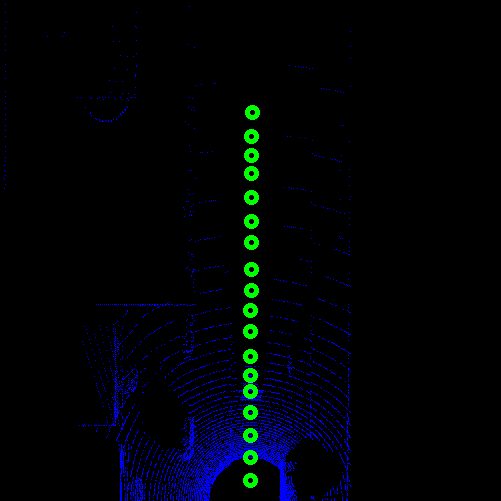
\includegraphics[scale=0.25]{../imgs/time_1.png} \label{t1}
    }
    \quad
    \subfigure[] {
        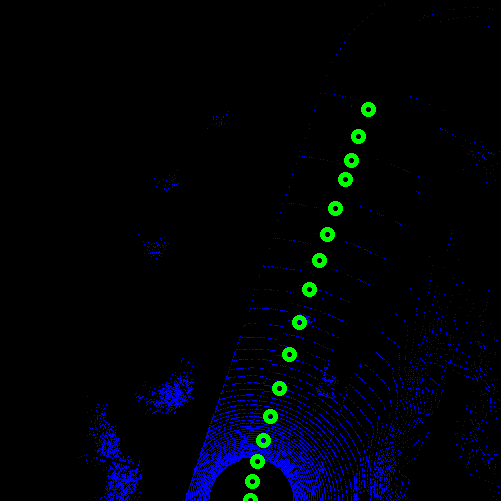
\includegraphics[scale=0.25]{../imgs/time_2.png} \label{t2}
    }
    \quad
    \subfigure[] {
        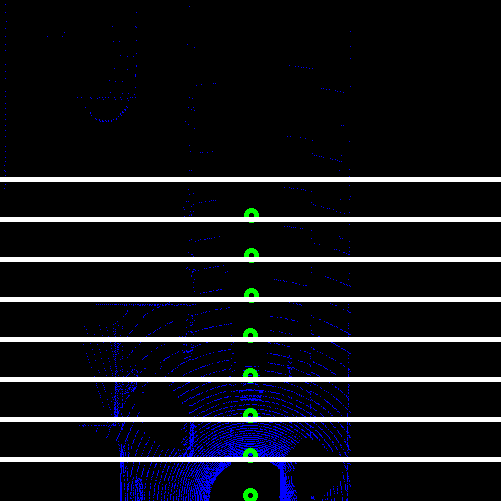
\includegraphics[scale=0.25]{../imgs/distance_1.png}\label{dis_1}
    }
    \quad
    \subfigure[] {
        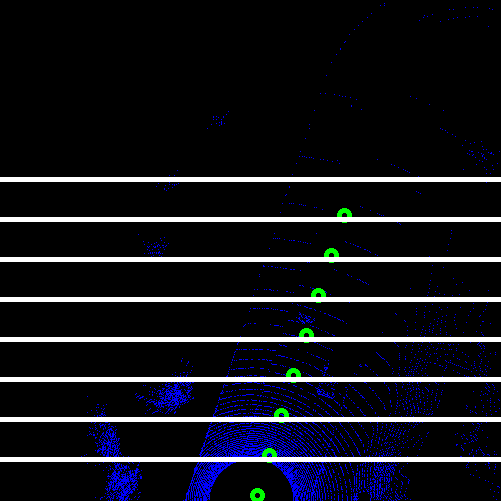
\includegraphics[scale=0.25]{../imgs/distance_2.png}\label{dis_2}
    }
    \caption{Several examples of the road main direction. The top two pictures are of the time-sampling method, and the bottom two pictures are of the  spatial-sampling method.}
    \label{representation}
\end{figure}
After projecting the results of global route planning to the road in the local LiDAR coordinate system, we use a series of key points $S=\{ p_1, p_2, \cdots , p_k\}, p_i=(x_i, y_i)$, where $x$ and $y$ indicate ``forward'' and ``left'' respectively in the LiDAR coordinate system, to represent the road main direction, which can be divided into two methods, time-sampling and spatial-sampling.

As shown in the Fig. \ref{t1} and \ref{t2}, we can project the historical trajectory points of the vehicle into the LiDAR coordinate system and then use the set of trajectory points to represent the road main direction.

This simple representation method is based on time-sampling. The time interval between every two points is equal. If the frequency of the odometer collecting the global coordinates is 50 Hz, the time interval between every two trajectory points is 20ms. The distance between every two trajectory points will be relatively close if the speed of the data-collecting vehicle is slow, otherwise will be relatively far. This leads to uneven data distribution, which is not conducive to model training.

Referring to the representation of lane line\cite{33}, another method to model road main direction is based on spatial-sampling, which is the method used in this article. Drawing several equally spaced horizontal lines under the bird's eye view of the point clouds, the road main direction is then represented by a set of intersections of the horizontal lines and the historical trajectory, as depicted in Fig. \ref{dis_1} and \ref{dis_2}. This method can generate uniformly distributed data compared to time-sampling method. The number of points can represent the length $l$ of the road main direction in appearance. Let the farthest observation distance be $H$ meters, spacing between these horizontal lines be $h$ meters, then the maximum length of the road main direction $M=\lfloor H/h \rfloor$. Because $h$ is fixed, these intersections can be uniquely determined by their y-coordinates, namely$\{y_0, y_1, \cdots, y_{l-1}\}$. 

For each horizontal line $h_s(x=x_s)$, finding the first trajectory point $p_i=(x_i, y_i)$ which x-coordinate is greater than $x_s$, then the index of the last trajectory point which x-coordinate is less than $x_s$ is $i-1$.Then we use the linear interpolation to obtain the corresponding y-coordinate $y_s$ of $x_s$ through (\ref{linear}):

\begin{equation} \label{linear}
    y_s = y_{i-1}-\frac{y_{i-1}-y_i}{x_{i-1}-x_i}(x_{i-1}-x_s), 
\end{equation}

Therefore, the road main direction can be represented as $D=\{l, y_0, y_1, \cdots, y_{l-1}, \cdots, y_M\}$, if $l<M$, the rest y-coordinates is set to zeros.

\subsection{Point Clouds Feature Extraction}
Our DirectionNet takes raw point clouds and noisy local navigation maps as input and output estimated main direction of the road, network architecture is shown in Fig. \ref{overview}.

There is no completely fixed paradigm for deep learning to process point clouds data. Several methods project point clouds into a perspective view to obtain BEV images or Range images\cite{34,35} and apply image-based feature extraction approaches. Some methods process point clouds directly\cite{36}. Considering the problem to be solved in this paper, extracting features from the bird's eye view\cite{12} is more in accordance with the physical meaning of the main direction of road.

DirectionNet takes two main steps to process the input LiDAR point clouds, just as shown in Fig. \ref{pfe}: (1) Rasterizing point clouds to 2D grids in Cartesian coordinates from the bird's eye view; (2) Converting the point clouds to the sparse pseudo-image through a Pillar feature net.

\begin{figure} 
    \centering
    \setlength{\belowcaptionskip}{-0.7cm}
    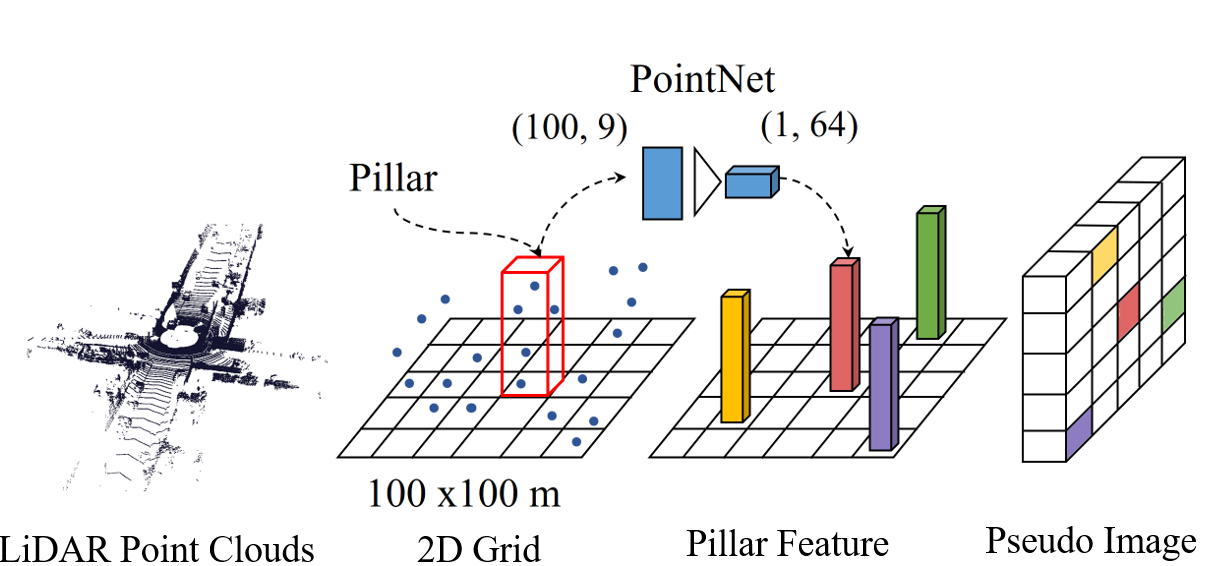
\includegraphics[width=\linewidth]{../imgs/pillar_feature_ex.png}
    \caption{\textbf{Pillar Feature Extractor:} We first discretize the point clouds into a 2D grid to generate a set of pillars, then use PointNet to extract pillar-wise features from these pillars.Finally, these pillar-wise features are scattered back to a 2D pseudo image.} 
    \label{pfe}
\end{figure}

\subsubsection{Point clouds Rasterization}
We first rasterize the point clouds into an evenly spaced grid on the $x-y$ plane, this is the same as cutting a series of pillars from the original 3D point clouds. We denote a point in the point clouds by $q=(x,y,z,r)$, where $x, y, z$ are 3D cartesian coordinates of $q$ and $r$ is the intensity. Same as in PointPillars\cite{12} and GndNet\cite{GND}, in addition to the 3D coordinates of the point, we apply feature enhancement on every point in each pillar by adding the offset relative to the centroid $c=(c_x,c_y,c_z)$ of all point clouds in the pillar: $x_c=(x-c_x), y_c=(y-c_y), z_c=(z-c_z)$, and the offset to the center of the pillar $x_p,y_p$. The point $q$ is enhanced from $D=4$ dimension to $D=9$ dimension.

Due to the sparsity of the point clouds, the pillars will be mostly empty, and the non-empty pillars usually have only a few points in. The number of non-empty pillars in each point clouds is different, and the number of points of each non-empty pillar is also different. For the batch training, we set the number of all the non-empty pillars from raw point clouds to $I$ and the number of points in each pillar to $N$, then we can get a fixed ($D, I, N$) size dense tensor after the rasterization. The data will be randomly sampled to the set size if the point clouds(pillars) contain too many pillars(points) or be padded by zero if the data is too little.

\subsubsection{Pillar Feature Extraction and Pseudo Image}
Next, we use a simplified version of PointNet which is the same as PointPillars\cite{12} and GndNet\cite{GND} to extract the point-wise feature of each non-empty pillar. The simplified PointNet consisting of a linear layer, BatchNorm\cite{bn} and ReLU generates a $(C_l, I, N)$ sized tensor, where the subscript $l$ indicates LiDAR. Then, a $(C_l, I)$ sized pillar-wise feature tensor is output through a max-pooling layer over the channels.

Last step, these pillar-wise features are projected to the original 2D grid map according to the grid coordinates of each pillar to obtain a $(C_l, H, W)$ sized pseudo-image, where $H$ and $W$ indicate the height and width of the 2D grid map.

\subsection{Attention Mechanism} \label{why_navg}
Because the vehicle will only travel in a fixed direction on the road instead of going in different directions at the same time, the method proposed in this paper only predicts one ``main direction" of the road. In most cases, this method is valid and accurate. However, in the cases of intersections, only using LiDAR point clouds as input, the predicted road main direction will be ambiguous because there is no navigational information about the direction of intersections. So we introduce the coarse precision navigation map to provide necessary navigational information to remove ambiguity at intersections.

We use one residual block of ResNet18 as the navigation feature extractor to process the input navigation map. The navigation feature extractor generates a $(C_m, H, W)$ sized feature map, where the subscript $m$ indicates navigation map. Then we concatenate the pseudo-image of size $(C_l, H, W)$ generated from LiDAR point clouds and the $(C_m, H, W)$ sized navigation feature map to get the fusion feature map of size $(C_f, H, W)$, where $f=l+m$.

Using this simple feature fusion method, the model may over-rely on the information of the navigation map and ignore the environmental information provided by the LiDAR point clouds. However, these noisy navigation maps are unreliable in many cases and the navigational information provided by these maps is not perfectly aligned with the main direction of the road. For the above considerations, we introduce the channel attention mechanism to learn the weights between navigation feature map and point clouds feature map, let neural network 
capture the correlations between navigation maps and LiDAR point clouds during fusion.

As shown in Fig. \ref{ca}, we first use both global-max-pooling and global-average-pooling simultaneously on the concatenated feature map $\mathrm{F}\in \mathbb{R}^{C\times H\times W}$ to aggregate two different spatial feature vectors: $\mathrm{F^{c}_{avg}}$ and $\mathrm{F^{c}_{max}}$. Both feature vectors are then fed into a weights-shared MLP with one hidden layer. In order to capture the relationship between different channels, the number of units in the hidden layer is set to $C/r$, where $r$ is the reduction rate. We then use element-wise addition to merge these two output feature vectors of the MLP. The channel attention map $\mathrm{M_c}\in \mathbb{R}^{C\times 1\times 1}$ is generated through a sigmoid activation function.This attention map represents the weights of different channels of the input feature map. Finally, using a channel-wise multiplication between $\mathrm{F_{c}}$ and $\mathrm{M_c}$ to get the channel attention weighted feature map $\mathrm{F^{\prime}}\in \mathbb{R}^{C\times H\times W}$.

In addition to the interference of intersections, dynamic vehicles on the road will also affect the prediction results of the model. So we introduce the spatial attention mechanism to let the model focus on the areas of interest such as road curbs or repeated objects on both sides of the road.

As shown in Fig. \ref{sa}, for the input feature map $\mathrm{F}\in \mathbb{R}^{C\times H\times W}$, we get two $(1, H, W)$ sized tensor from channel-average-pooling and channel-max-pooling and then concatenate them along the channel axis to highlight focus regions. After pooling, we apply a 2D convolution layer with sigmoid activation function on the $(2, H, W)$ sized concatenated tensor to generate the spatial attention map $\mathrm{M_s}\in \mathbb{R}^{1\times H\times W}$. Finally, using multiplication between $\mathrm{F_{in}}$ and $\mathrm{M_s}$ to get the spatial attention weighted feature map $\mathrm{F^{\prime}}\in \mathbb{R}^{C\times H\times W}$.

Similar with CBAM\cite{CBAM}, we connect channel attention block and spatial attention block in series (as depicted in Fig. \ref{connect}) to focus on `which' is imporant between navigation maps and LiDAR point clouds, `where' is important on the road.

Once getting the refined fused feature through the attention block, we can use a 2D backbone such as ResNet\cite{37} to extract the high-level feature map and a full-connected layer to regress the length and y-coordinates representing the road main direction.

\begin{figure}
    \centering
    \setlength{\belowcaptionskip}{-0.6cm}
    \subfigure[Channel Attention Block] {
        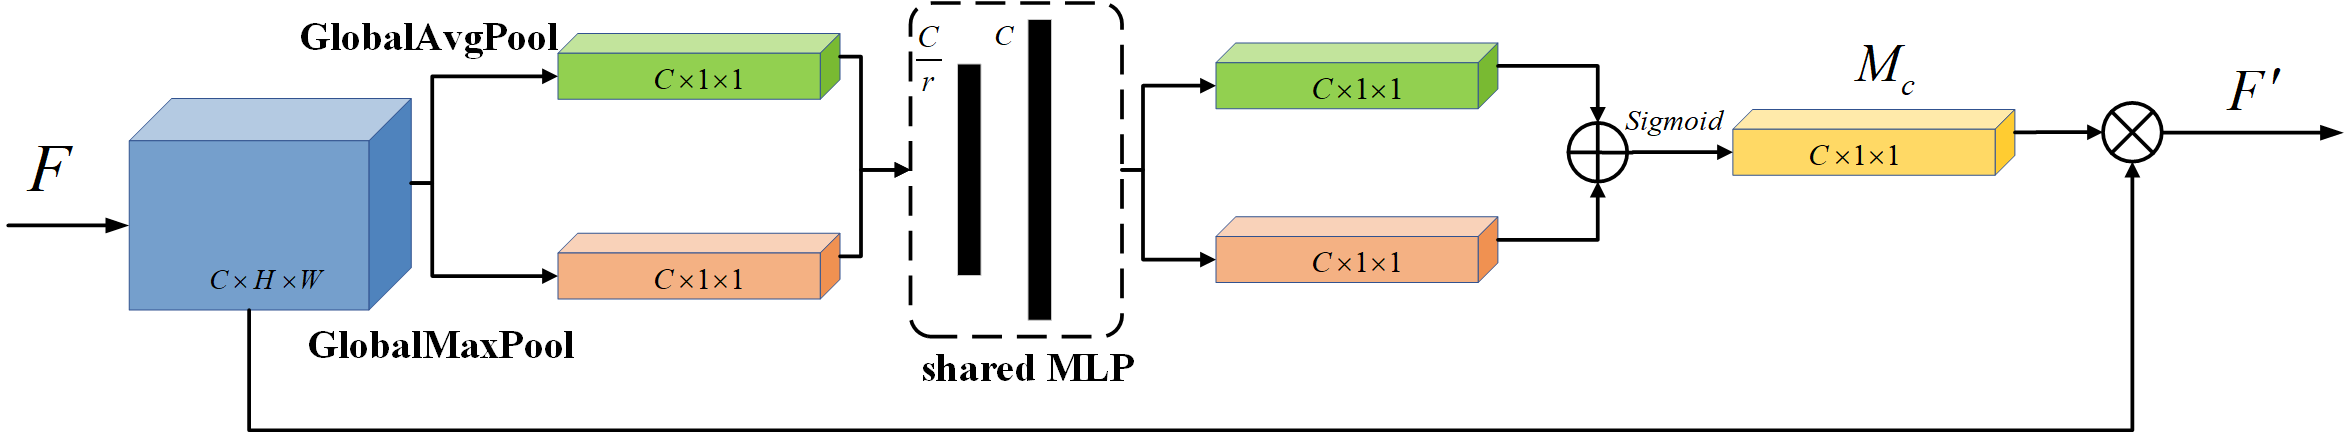
\includegraphics[width=\linewidth]{../imgs/attention_1.png}\label{ca}
    }
    \subfigure[Spatial Attention Block] {
        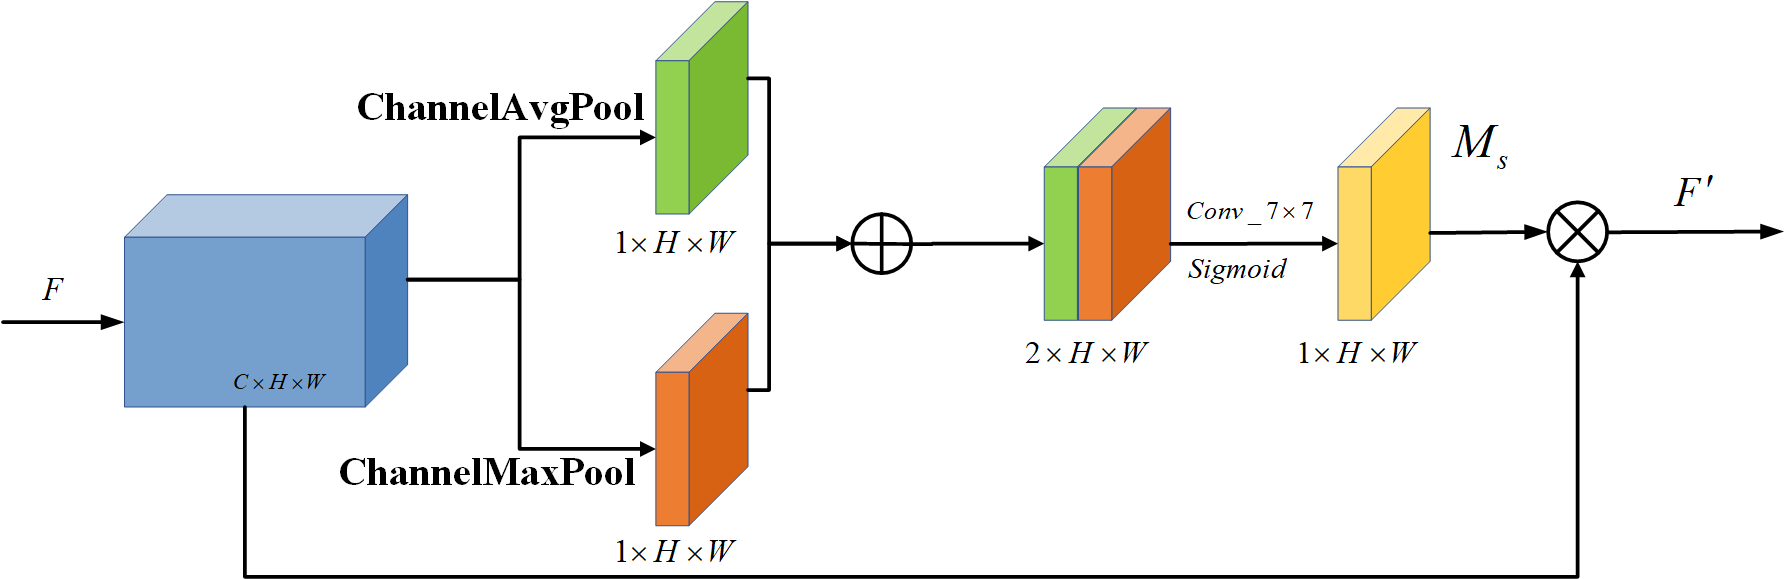
\includegraphics[width=\linewidth]{../imgs/attention_2.png}\label{sa}
    }
    \subfigure[Connect CAB and SAB in series] {
        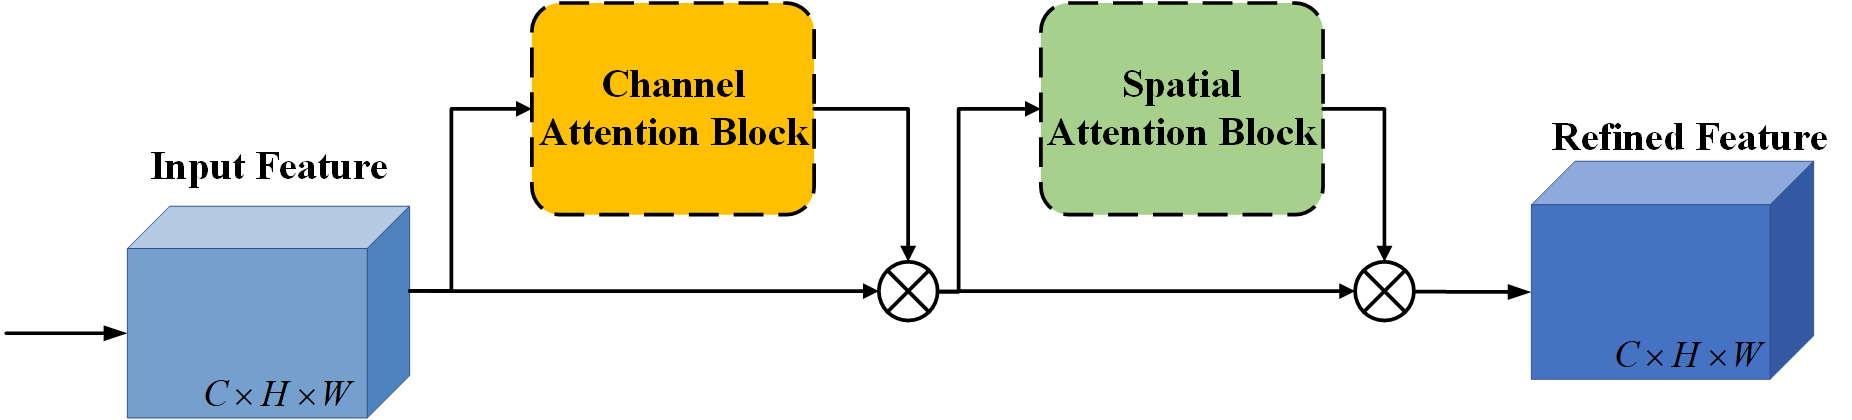
\includegraphics[width=\linewidth]{../imgs/conect.png}\label{connect}
    }
    \caption{\textbf{The overview of the attention mechanism.} \textbf{(a):} The channel attention uses both global-average-pooling and global-max-pooling following with a shared MLP to merge information between channels; \textbf{(b):} The spatial attention utilizes both channel-average-pooling and channel-max-pooling following with a convolution layer to obtain spatial information; \textbf{(c):} Finally, connect channel attention block and spatial attention block in series.}
\end{figure}

\subsection{Loss Function}
We train the DirectionNet using an $L_2$ loss between the predicted road main direction $D_t^p$ and the ground truth road main direction $D_t^{gt}$ at the $t$-th frame, then the loss function is given by:
\begin{equation}
    \mathcal{L}=||D_t^p-D_t^{gt}||_2, 
\end{equation}
Note that if the ground truth length of the road main direction $l_t^{gt}$ is less than the maximum length $M$ of the road main direction, the rest loss is set to zeros.

\section{EXPERIMENTS}\label{experiments}

\subsection{Data Collection}
It's very easy to obtain the training data for our DirectionNet and don't need manual data annotation. Only a vehicle with LiDAR is required, odometry information can be provided by wheel odometer, Lidar SLAM technology or GPS. In this part, we use the CARLA\cite{CARLA} simulator to generate the dataset. We use Town04 to Town06 as training and hold out Town03 for validation, all of these towns are US style. We generate local navigation map by drawing all routes white on black background and drawing red on the traversed roads to simulate the results of global planning.

\subsection{Data Processing and Augmentation}

For each point cloud, the points within 2m from the LiDAR are removed due to the occlusion of data-collecting vehicle. We apply a number of data augmentations during training to expose the model to novel cases that are not collected and enhance the generalization performance of the model.

Firstly, we randomly rotate the point clouds and the road main direction points by a random yaw angle $\theta \in\pm10 \degree$ to simulate the situation of the front of the car facing different directions on the road. This enables the model to pull the vehicle back to the main direction of the road. Then randomly horizontal flipping the point clouds and the corresponding road main direction points to simulate different turning directions out of the intersection. Besides, we add Gaussian noise on the navigation map to enhance the robustness of the system.

\subsection{Implementation Details}
We rasterize the point cloud into a $(50m\times50m)$ sized 2D grid map, the cell resolution is $(0.5m\times0.5m)$ , so $H=W=100$. The $x, y, z$ axes are in the range of $[(0m, 50m),(-25m, 25m),(-4m, 4m)]$ and the points outside the range will be removed. The maximum number of points per pillar $(N)$ is 100 and the maximum number of pillars per point cloud ($I$) is 10000.

The farthest observation distance $H$ is set to 20 meters, spacing between these horizontal lines $h$ is set to 0.5 meter.

The model is implemented in TensorFlow\cite{tensorflow2015-whitepaper} and the training data is converted into TFRecord to accelerate the training.

\subsection{Evaluation Metrics}
For algorithm evaluation, we design two evaluation metrics, stability and accuracy. Stability is used to evaluate the reliability of the method, which is critical in autonomous driving systems. Only if there are enough prediction points, the prediction result can reflect the direction of the road. One prediction is considered valid if the prediction length $l>\delta_l $. Accuracy is used to evaluate how well the valid predicted direction aligns with the true direction. The definitions of these measures are as follows:

\begin{equation}
    Stability = \frac{N_{valid}}{N_{total}}, \quad Accuracy_i=\frac{C_i}{S_i}, 
\end{equation}
where $N_{valid}$ is the number of the valid predictions, $N_{total}$ is the number of all predictions, $C_i$ indicates the number of correctly predicted trajectory points in the prediction result of the i-th frame, and $S_i$ represents the minimum of the predicted length and the ground-truth length.

If the distance between the ground-truth y-coordinate offset and the predicted offset is less than a given threshold (e.g. 0.5 meter), the predicted offset is assumed to be correct.

\subsection{Results}
\subsubsection{Performance on CARLA}
Our DirectionNet can get an average accuracy of $86.6\%$ and $100\%$ stability on the validation set. Note that, we use the autopilot script provided by CARLA to collect data for training and testing, this script will control the vehicle to do some actions such as obstacles avoiding and lanes chaning. Because of this, the collected historical trajectory points will not perfectly align with the real main direction of the road, so the average accuracy on the validation set will be lower than the actual result.

Real-time is very important for the autonomous driving systems. Our model can process each frame of data within 60ms, which can fully meet the real-time requirement. The specific performance is shown in Fig. \ref{withmap}. From which we can see that no matter driving on the stright/curve road or at the intersections, our DirectionNet can predict the main direction of the road correctly and stably. With the LiDAR point clouds and local navigation map, the predicted road main direction can guide the vehicle drive to the the destination along the road.
\begin{figure}[]
    \centering
    \setlength{\belowcaptionskip}{-0.5cm}
    \subfigure[] {
        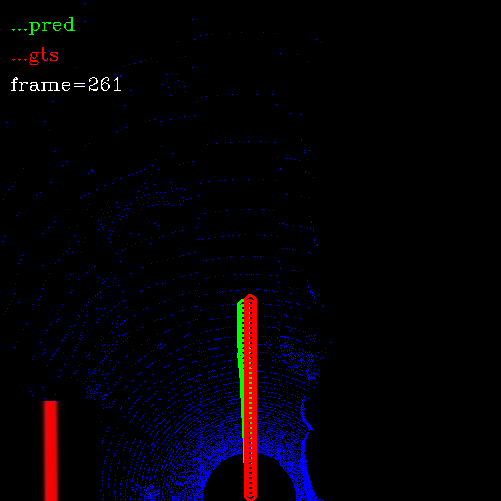
\includegraphics[scale=0.25]{../imgs/withmap_line.png}
    }
    \quad
    \subfigure[] {
        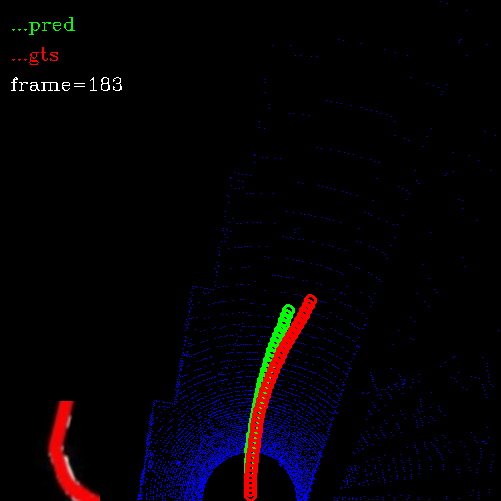
\includegraphics[scale=0.25]{../imgs/withmap_curve.png}
    }
    \quad
    \subfigure[] {
        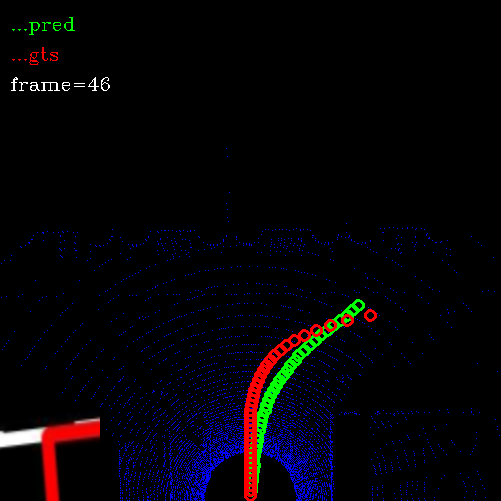
\includegraphics[scale=0.25]{../imgs/withmap_inter_46.png}
    }
    \quad
    \subfigure[] {
        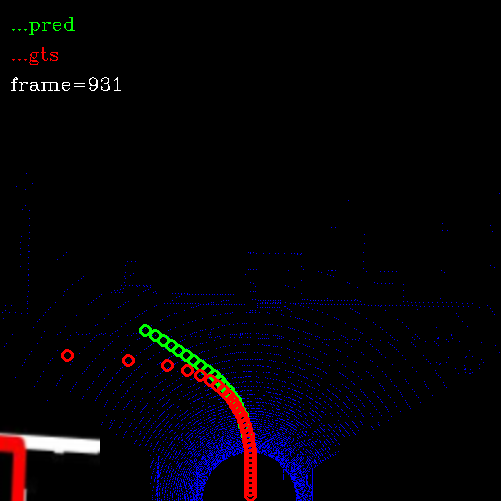
\includegraphics[scale=0.25]{../imgs/withmap_inter_931.png}
    }
    \caption{Several results on the CARLA. The top two pictures are at straight roads, and the bottom two pictures are at intersections.Green points indicate the predicted road main direction and red points indicate the ground truth.}
    \label{withmap}
\end{figure}

\subsubsection{Ablation Experiments}
To verify the influence of the navigation map and attention mechanism on our proposed model, we performed several ablation experiments. Firstly, we make two groups of controlled experiments to figure out what role the navigation map plays in our model.

In one controlled experiment, we set the input navigation maps to zeros to observe the prediction results only using the LiDAR point clouds, the result is shown in Fig. \ref{without_navg_map}. Without the navigation maps,our DirectionNet can still correctly predict the road main direction on the stright/curve road. However, just as mentioned in Section \ref{why_navg}, the predicted road main direction will be ambiguous at intersections since there is no information of which direction to go. As expected, the navigation maps provide the model with necessary navigational information to remove ambiguity at intersections.

\begin{figure}
    \centering
    \setlength{\belowcaptionskip}{-0.5cm}
    \subfigure[] {
        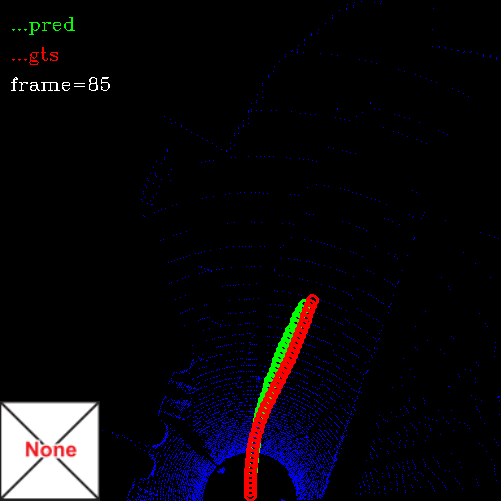
\includegraphics[scale=0.25]{../imgs/without_map_2.png}
    }
    \quad
    \subfigure[] {
        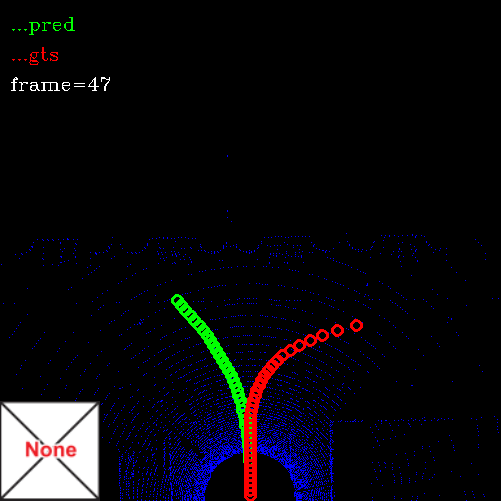
\includegraphics[scale=0.25]{../imgs/without_map_1.png}
    }
    \subfigure[] {
        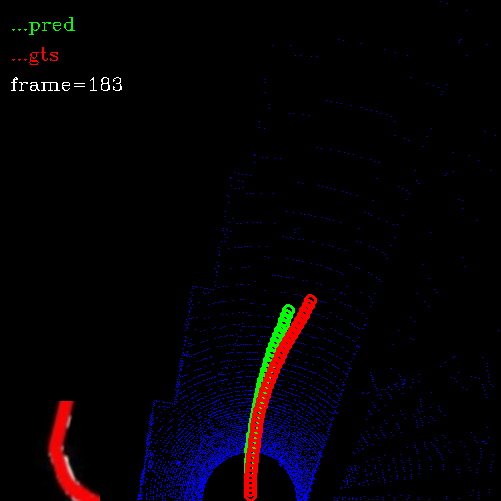
\includegraphics[scale=0.25]{../imgs/withmap_curve.png}
    }
    \quad
    \subfigure[] {
        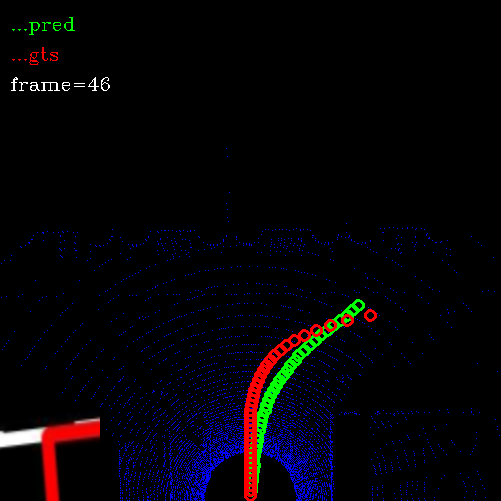
\includegraphics[scale=0.25]{../imgs/withmap_inter_46.png}
    }
    \caption{The results of controlled experiments w/ and w/o navigation maps. The top two pictures are w/o navigation maps, and the bottom are w/ navigation maps.}
    \label{without_navg_map}
\end{figure}

In another controlled experiment, we fix the input navigation map as ``turning-left'' to check if the navigation maps are over trusted. Just as shown in Fig. \ref{set_0} and \ref{set_1}, when driving on the stright road, although the navigation map gives a wrong turning-left signal, the predicted road main direction is still stright. But at the intersection, in Fig. \ref{set_2} and \ref{set_3}, the prediction direction will inevitably turn left. From this, we can conclude that our DirectionNet does not rely too much on the navigation map, but will combine the environmental information provided in the LiDAR point cloud and the navigational information to give the final prediction.

\begin{figure}
    \centering
    \setlength{\belowcaptionskip}{-0.5cm}
    \subfigure[] {
        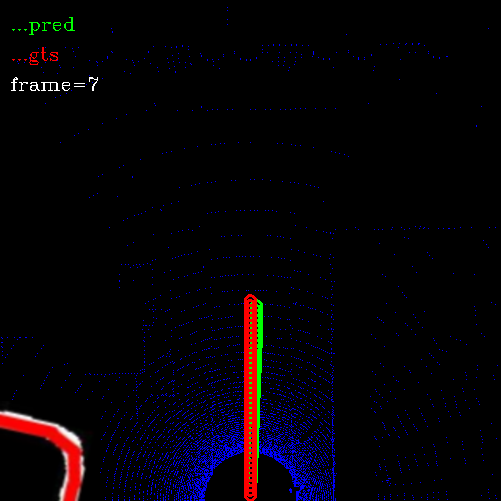
\includegraphics[scale=0.25]{../imgs/set_map_stight_2.png} \label{set_0}
    }
    \subfigure[] {
        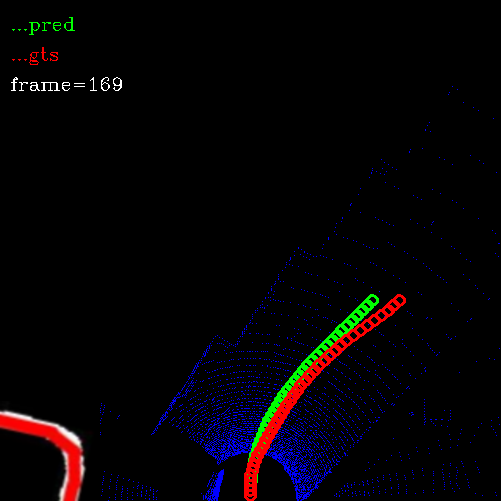
\includegraphics[scale=0.25]{../imgs/set_map_stight.png} \label{set_1}
    }
    \subfigure[] {
        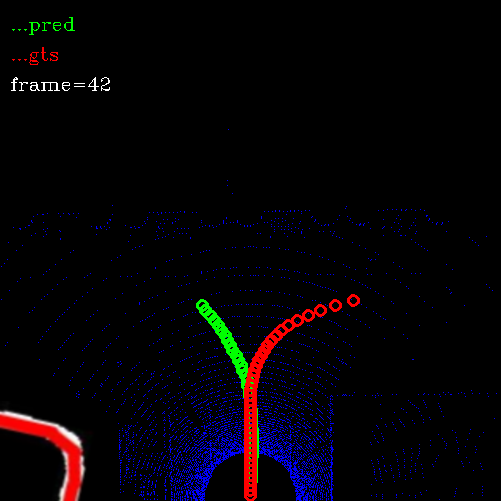
\includegraphics[scale=0.25]{../imgs/set_map_inter_1.png} \label{set_2}
    }
    \subfigure[] {
        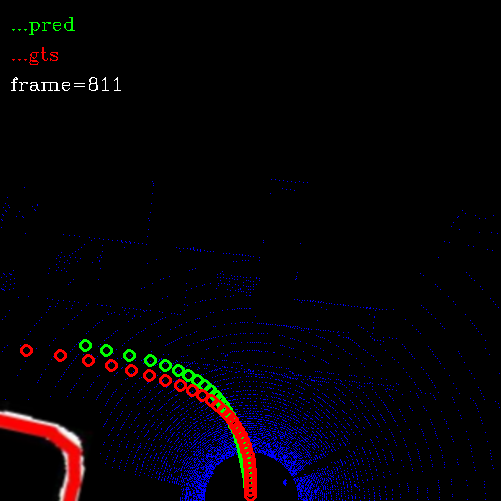
\includegraphics[scale=0.25]{../imgs/set_map_inter_2.png} \label{set_3}
    }
    \caption{The results of controlled experiments of fixed ``turning-left'' input navigation map. The top two pictures are at straight roads, and the bottom two pictures are at intersections.}
    \label{set_navg_map}
\end{figure}

Secondly, we make one group of controlled experiments to figure out how the spatial attention mechanism affects model performance, the result is shown in Fig. \ref{without_spa_att}. We can clearly see that the predicted direction will be severely affected by the obstacles on the road without spatial attention mechanism and this phenomenon is effectively improved after adding the spatial attention mechanism.

\begin{figure}
    \centering
    \setlength{\belowcaptionskip}{-0.6cm}
    \subfigure[W/O Spatial Attention] {
        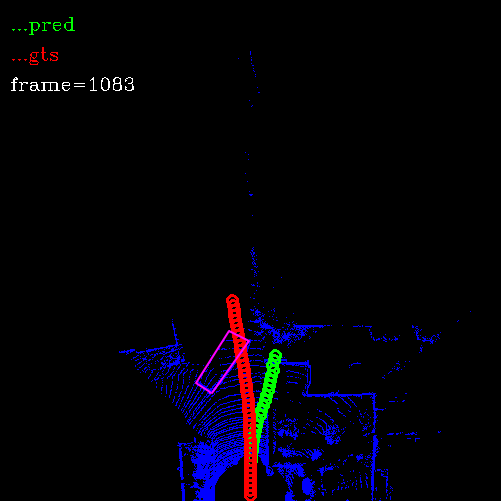
\includegraphics[scale=0.25]{../imgs/obs_without_att_2.png}
    }
    \quad
    \subfigure[W/ Spatial Attention] {
        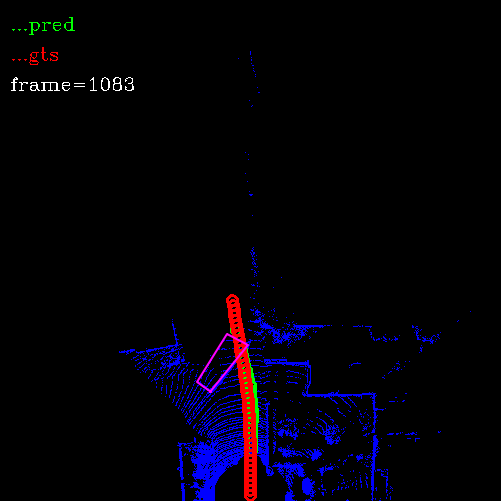
\includegraphics[scale=0.25]{../imgs/obs_with_att.png}
    }
    \caption{The results of controlled experiments w/ and w/o spatial attention mechanism.In the pink box is the obstacle in front of the road.}
    \label{without_spa_att}
\end{figure}

\subsubsection{Generalization Experiments}
Although the method proposed in this paper has shown good performance in the simulation environment, it is a big challenge to deploy the method on real-word vehicles with a variety of installed LiDARs. To test the generalization performance of the model, we first test the model trained with CARLA simulated data on the KITTI\cite{38,39} odometry dataset which is collected in real-world. The average accuracy dropped from $86.6\%$ to $83.3\%$. Because the LiDAR used in both of CARLA and KITTI is 64-channel mechanical LiDAR, the drop of performance is not noticeable. 

But when we test the model on a 128-channel mechanical LiDAR, the performance has dropped so dramatically that the predicted road direction no longer reflect the direction of the road at all. The results can be found in Fig. \ref{sim2rel}. Therefore, enhancing the generalization ability of our proposed method on LiDARs with different scanning patterns will be the focus of the future study.

\begin{figure}
    \centering
    \setlength{\belowcaptionskip}{-0.5cm}
    \subfigure[KITTI result] {
        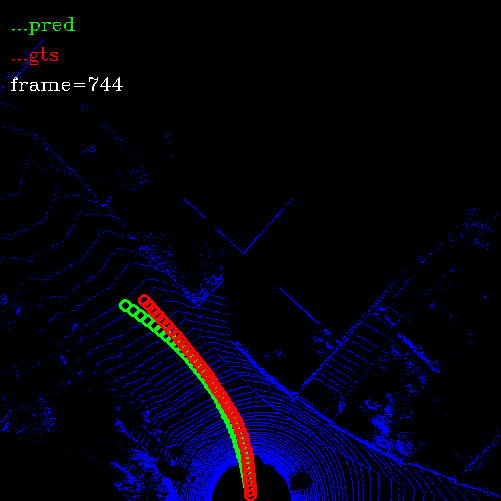
\includegraphics[scale=0.25]{../imgs/car2kitti.png}
    }
    \quad
    \subfigure[128-channel LiDAR] {
        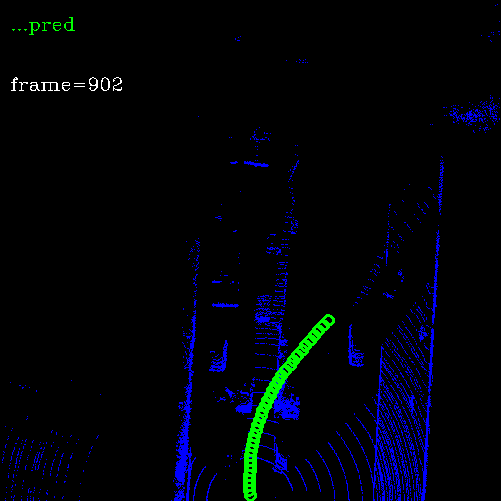
\includegraphics[scale=0.25]{../imgs/128_2.png}
    }
    \caption{The results of generalization performance test (We don't have ground truth of the 128-channel LiDAR).}
    \label{sim2rel}
\end{figure}

There is a growing trend for the autonomous driving companies to use more and more cheap solid-state LiDARs instead of expensive traditional mechanical scanning LiDARs. Therefore, we also test the generalization performance of the model on the solid-state LiDAR, the results can be seen in Fig. \ref{livox}. The performance also dropped dramatically.

\begin{figure}
    \centering
    \setlength{\belowcaptionskip}{-0.5cm}
    \subfigure[]{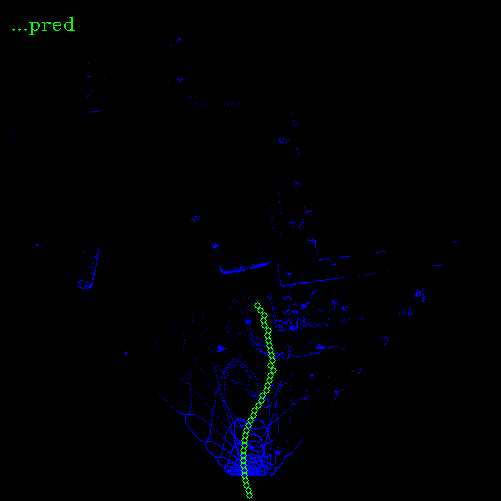
\includegraphics[scale=0.25]{../imgs/BEV_livox31.png}}
    \subfigure[]{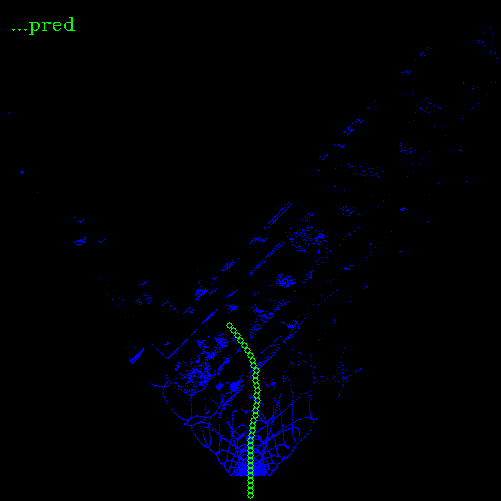
\includegraphics[scale=0.25]{../imgs/BEV_livox_4.png}}
    \caption{The results of generalization performance test on the solid-state LiDAR.}
    \label{livox}
\end{figure}

In conclusion, our model can still work normally on the LiDARs with similar scanning patterns, but cannot work with LiDARs with different scanning patterns.

\section{CONCLUSIONS}\label{conclusions}
In this paper, we find an intermediate way to transit from traditional autonomous driving methods to end-to-end autonomous driving methods to fully exploit the strengths of deep learning. Inspired by human's driving style, the proposed DirectionNet can extract the road main direction of the road directly from the LiDAR point clouds, which can be used with subsequent motion planning and control to guide the vehicle drive along the road.

Up to now, the generalization ability of our method is not suitable for LiDARs with different scanning patterns on the market. Though collecting more training data from different LiDAR and training a new model from scratch could alleviate this problem, it unfortunately might be infeasible due to various LiDARs and real-world scenarios. Thus, our future work will tend to utilize domain adaptation technology\cite{DA} to enhance the generalization ability of our method under different LiDARs and different geographic environments.
\addtolength{\textheight}{-0cm}
\bibliographystyle{../IEEEtranBST/IEEEtran}
\bibliography{../IEEEtranBST/IEEEabrv,../ref/my_lib.bib}
\end{document}
